

\title{Statistical Inference In Application Of Real World Data}

\author{David Plotz\\
Ambica Nandimandalam\\
Patrick Sorgaard \\
\vspace{5mm}
California State University East Bay\\
Statistic Department\\
Professor Shenghua Fan}

\begin{document}

\begin{frame}
\titlepage
\end{frame}

\begin{frame}{Fisher's Iris Data}
\indent Consider the following data set, often consider \emph{Fisher's Iris Data Set}, which is a multivariate data set representing four different variables for three different species of Iris.\\
\begin{table}
\begin{center}
\scalebox{0.75}{
\begin{tabular}{|c|c|c|c|l|}
\hline
\textbf{Sepal Length} & \textbf{Sepal Width} & \textbf{Petal Length} & \textbf{Petal Width} & \textbf{\hspace{1.5mm}Species} \\
\hline
$5.1_{{}_{1}}$ & $3.5_{{}_{1}}$	& $1.4_{{}_{1}}$ & $0.2_{{}_{1}}$ & \emph{I. setosa}\\
\hline
\vdots & \vdots & \vdots & \vdots & \vdots\\
\hline
$5.0_{{}_{50}}$ & $3.3_{{}_{50}}$ & $1.4_{{}_{50}}$ & $0.2_{{}_{50}}$ & \emph{I. setosa}\\
\hline
$7.0_{{}_{1}}$ & $3.2_{{}_{1}}$	& $4.7_{{}_{1}}$ & $1.4_{{}_{1}}$ & \emph{I. versicolor}\\
\hline
\vdots & \vdots & \vdots & \vdots & \vdots\\
\hline
$5.7_{{}_{50}}$ & $2.8_{{}_{50}}$ & $4.1_{{}_{50}}$ & $1.3_{{}_{50}}$ & \emph{I. versicolor}\\
\hline
$6.3_{{}_{1}}$ & $3.3_{{}_{1}}$	& $6.0_{{}_{1}}$ & $2.5_{{}_{1}}$ & \emph{I. virginica}\\
\hline
\vdots & \vdots & \vdots & \vdots & \vdots\\
\hline
$5.9_{{}_{50}}$ & $3.0_{{}_{50}}$ & $5.1_{{}_{50}}$ & $1.8_{{}_{50}}$ & \emph{I. virginica}\\
\hline
\end{tabular}}
\end{center}
\end{table}
\end{frame}

\begin{frame}
We'll consider this data set as a representative of real world data, which we must note was collected by Edgar Anderson in order to measure the morphological variation of three different species of Iris.\\
\centerline{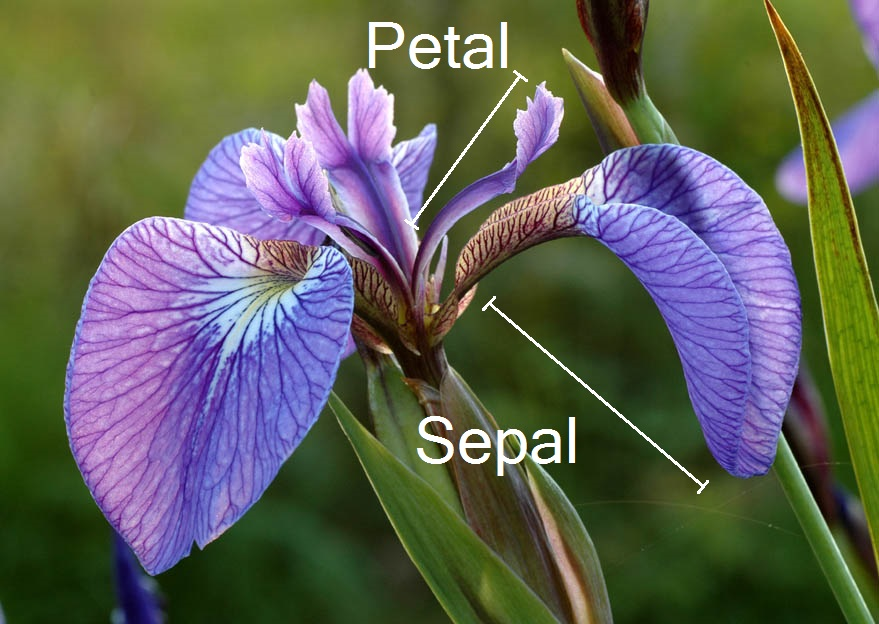
\includegraphics[width=6cm]{Iris-setosa-1.jpg}}
\centerline{An example of the species \emph{I. setosa}.}
 Note that the measurement samples were collected on the same day, in the same pasture and with the same instrument, hence we assume the samples are independent and identically distributed.
\end{frame}

\begin{frame}{Descriptive Statistics}
The following is a table for the mean $\bar{x}_{ij}$ and standard deviation $s_{ij}$ for the four variables between the three species.

\vspace{2mm}
\centerline{\scalebox{0.6}{
\begin{tabular}{|c|c|c|c|l|}
\hline
\textbf{Sepal Length} & \textbf{Sepal Width} & \textbf{Petal Length} & \textbf{Petal Width} & \textbf{\hspace{1.5mm}Species} \\
\hline
$\bar{x}_{11}=5.006$, $s_{11}=0.3525$ & $\bar{x}_{12}=3.428$, $s_{12}=0.3791$	& $\bar{x}_{13}=1.462$, $s_{13}=0.0246$ & $\bar{x}_{14}=0.246$, $s_{14}=0.1054$ & \emph{I. setosa}\\
\hline
$\bar{x}_{21}=5.936$, $s_{21}=0.5162$ & $\bar{x}_{22}=2.77$, $s_{22}=0.0444$ & $\bar{x}_{23}=4.26$, $s_{23}=0.4699$ & $\bar{x}_{24}=1.326$, $s_{24}=0.1978$ & \emph{I. versicolor}\\
\hline
$\bar{x}_{31}=6.588$, $s_{31}=0.6359$ & $\bar{x}_{32}=2.974$, $s_{32}=0.0456$	& $\bar{x}_{33}=5.552$, $s_{33}=0.078$ & $\bar{x}_{34}=2.026$, $s_{34}=0.2747$ & \emph{I. virginica}\\
\hline
\end{tabular}}}

\vspace{2mm}
Using $\alpha=0.05$ with $z_{{}^{\alpha}/_2}=1.96$, we get the following $95\%$ confidence intervals, $\bar{x}_{ij}\pm z_{{}^{\alpha}/_2}\frac{s_{ij}}{\sqrt{n}}$.

\vspace{2mm}
\centerline{\scalebox{0.6}{
\begin{tabular}{|c|c|c|c|l|}
\hline
\textbf{Sepal Length} & \textbf{Sepal Width} & \textbf{Petal Length} & \textbf{Petal Width} & \textbf{\hspace{1.5mm}Species} \\
\hline
$\left(\text{4.90829},\text{5.10371}\right)_{11}$ & $\left(\text{3.32292},\text{3.53308}\right)_{12}$	& $\left(\text{1.41385},\text{1.51015}\right)_{13}$ & $\left(\text{0.216785},\text{0.275215}\right)_{14}$ & \emph{I. setosa}\\
\hline
$\left(\text{5.79292},\text{6.07908}\right)_{21}$ & $\left(\text{2.68302},\text{2.85698}\right)_{22}$ & $\left(\text{4.12975},\text{4.39025}\right)_{23}$ & $\left(\text{1.27117},\text{1.38083}\right)_{24}$ & \emph{I. versicolor}\\
\hline
$\left(\text{6.41174},\text{6.76426}\right)_{31}$ & $\left(\text{2.88461},\text{3.06339}\right)_{32}$	& $\left(\text{5.39902},\text{5.70498}\right)_{33}$ & $\left(\text{1.94986},\text{2.10214}\right)_{34}$ & \emph{I. virginica}\\
\hline
\end{tabular}}}

\vspace{2mm}
Hence we are $95\%$ confident that the true population parameter $\mu$ of each variable for each species of Iris is between $x_{ij}-1.96\cdot\frac{s_{ij}}{\sqrt{50}}$ and $x_{ij}+1.96\cdot\frac{s_{ij}}{\sqrt{50}}$ centimeters.
\end{frame}

\begin{frame}
\centerline{\includegraphics[width=12cm]{VariableBoxPlot}}
\end{frame}

\begin{frame}
\centerline{\includegraphics[width=6cm]{SepalLengthHistogram.png}\includegraphics[width=6cm]{SepalWidthHistogram.png}}
\centerline{\includegraphics[width=6cm]{PetalLengthHistogram.png}\includegraphics[width=6cm]{PetalWidthHistogram.png}}
\end{frame}

\begin{frame}{Tests For Comparing Means}
We consider the previous histograms as a way to analyze the distributions of the Iris species  within each variable. 

\vspace{2mm}
$\bullet$ We can see that the distributions for each of the species are relatively unimodal, but most of the distributions are relatively skewed, although they could pass for normal.

\vspace{2mm}
$\bullet$ Note that even if each distribution is non-normal, by the Central Limit Theory as long as each random variable is standardized and has sample size $n\geq 30$, the behavior of the random variable will be approximately normal. Hence a comparative test for equal means is applicable for every one of the distributions since each distribution contains sample size $n=50$.

\vspace{2mm}
$\bullet$ Note that the actual parameter $\sigma$ is unknown, hence we must consider the $t$ approximation making use of $s$.
\end{frame}

\begin{frame}
Before determining which distributions have similar distributions, the type of test for equal variances used depends on the normality of the distribution. The following is a table of results of the hypothesis with significance $\alpha=0.5$,
$$H_0:\hspace{1mm}\text{The distribution is normal.}\hspace{1mm}H_a:\hspace{1mm}\text{The distribution is non-normal.}$$
\centerline{\scalebox{0.6}{
\begin{tabular}{|c|c|c|c|}
\hline
\textbf{Distribution} & \textbf{$p$-value} & \textbf{Choice} & \textbf{Normality}\\
\hline
Sepal Length \emph{I. setosa} & 0.335 & Fail to reject $H_0$. & Normal \\
\hline
Sepal Length \emph{I. versicolor} & 0.433 & Fail to reject $H_0$ & Normal \\
\hline
Sepal Length \emph{I. virginica} & 0.148 & Fail to reject $H_0$. & Normal \\
\hline
Sepal Width \emph{I. setosa} & 0.21 & Fail to reject $H_0$. & Normal \\
\hline
Sepal Width \emph{I. versicolor} & 0.141 & Fail to reject $H_0$. & Normal \\
\hline
Sepal Width \emph{I. virginica} & 0.102 & Fail to reject $H_0$. & Normal \\
\hline
Petal Length \emph{I. setosa} & 0.011 & Reject $H_0$. & Non-normal \\
\hline
Petal Length \emph{I. versicolor} & 0.145 & Fail to reject $H_0$. & Normal \\
\hline
Petal Length \emph{I. virginica} & 0.107 & Fail to reject $H_0$. & Normal \\
\hline
Petal Width \emph{I. setosa} & $<$0.005 & Reject $H_0$. & Non-normal \\
\hline
Petal Width \emph{I. virsicolor} & 0.014 & Reject $H_0$. & Non-normal \\
\hline
Petal Width \emph{I. virginica} & 0.051	& Fail to reject $H_0$. & Normal \\
\hline
\end{tabular}}}
\end{frame}

\begin{frame}
Making proper use of the $t$ approximation requires determining whether comparative distributions have a similar $s$. The following is a table showing the results of the hypothesis with significance $\alpha=0.05$,
$$H_0:\hspace{1mm}\sigma^2_{i}=\sigma^2_{j},\hspace{1mm}H_a:\hspace{1mm}\sigma^2_{i}\centernot{=}\sigma^2_{j},\hspace{1mm}i\centernot{=}j.$$
\centerline{\scalebox{0.6}{
\begin{tabular}{|c|c|c|c|}
\hline
\textbf{Tested Deviations} & \textbf{$p$-value} & \textbf{Choice} & \textbf{Outcome}\\
\hline
Sepal Length: \emph{I. setosa} / \emph{I. versicolor} & 0.009 & Reject $H_0$. & $\sigma^2_{{}_{setosa}}\centernot{=}\sigma^2_{{}_{versicolor}}$ \\
\hline
Sepal Length: \emph{I. setosa} / \emph{I. virginica} & 0.000 & Reject $H_0$. & $\sigma^2_{{}_{setosa}}\centernot{=}\sigma^2_{{}_{virginica}}$ \\
\hline
Sepal Length: \emph{I. versicolor} / \emph{I. virginica} & 0.148 & Fail to reject $H_0$. & $\sigma^2_{{}_{versicolor}}=\sigma^2_{{}_{virginica}}$ \\
\hline
Sepal Width: \emph{I. setosa} / \emph{I. versicolor} & 0.189 & Fail to reject $H_0$. & $\sigma^2_{{}_{setosa}}=\sigma^2_{{}_{versicolor}}$ \\
\hline
Sepal Width: \emph{I. setosa} / \emph{I. virginica} & 0.261 & Fail to reject $H_0$. & $\sigma^2_{{}_{setosa}}=\sigma^2_{{}_{virginica}}$ \\
\hline
Sepal Width: \emph{I. versicolor} / \emph{I. virginica} & 0.849 & Fail to reject $H_0$. & $\sigma^2_{{}_{versicolor}}=\sigma^2_{{}_{virginica}}$ \\
\hline
${}^*$Petal Length: \emph{I. setosa} / \emph{I. versicolor} & 0.000 & Reject $H_0$. & $\sigma^2_{{}_{setosa}}\centernot{=}\sigma^2_{{}_{versicolor}}$ \\
\hline
${}^*$Petal Length: \emph{I. setosa} / \emph{I. virginica} & 0.000 & Reject $H_0$. & $\sigma^2_{{}_{setosa}}\centernot{=}\sigma^2_{{}_{virginica}}$ \\
\hline
Petal Length: \emph{I. versicolor} / \emph{I. virginica} & 0.264 & Fail to reject $H_0$. & $\sigma^2_{{}_{versicolor}}=\sigma^2_{{}_{virginica}}$ \\
\hline
${}^*$Petal Width: \emph{I. setosa} / \emph{I. versicolor} & 0.000 & Reject $H_0$. & $\sigma^2_{{}_{setosa}}\centernot{=}\sigma^2_{{}_{versicolor}}$ \\
\hline
${}^*$Petal Width: \emph{I. setosa} / \emph{I. virginica} & 0.000 & Reject $H_0$. & $\sigma^2{{}_{setosa}}\centernot{=}\sigma^2_{{}_{virginica}}$ \\
\hline
${}^*$Petal Width: \emph{I. versicolor} / \emph{I. virginica} & 0.012 & Reject $H_0$. & $\sigma^2_{{}_{versicolor}}\centernot{=}\sigma^2_{{}_{virginica}}$ \\
\hline
\end{tabular}}}

\vspace{2mm}
${}^*$ denotes a non-normal distribution and use a of non $F$-test. 
\end{frame}

\begin{frame}
Along with the previous results we can now make use of a comparative mean $t$-test. With $t$-test for independent means and $\sigma^2_1=\sigma^2_2$:
$$t=\frac{\bar{y}_1-\bar{y}_2-D_0}{s_p\sqrt{\frac{1}{n_1}+\frac{1}{n_2}}},\hspace{1mm}df=n_1+n_2-2,$$
or $t'$-test for independent means and $\sigma^2_1\centernot{=}\sigma^2_2$ where $c=\frac{\frac{s^2_1}{n_1}}{\frac{s^2_1}{n_1}+\frac{s^2_2}{n_2}}$:
$$t'=\frac{\bar{y}_1-\bar{y}_2-D_0}{\sqrt{\frac{s^2_1}{n_1}+\frac{s^2_2}{n_2}}},\hspace{1mm}df=\frac{\left(n_1-1\right)\left(n_2-1\right)}{\left(1-c\right)^2\left(n_1-1\right)+c^2\left(n_2-1\right)}.$$
Making use of these tests, we get the following table of results for the hypothesis with significance $\alpha=0.05$,
$$H_0:\hspace{1mm}\mu_i=\mu_j,\hspace{1mm}H_a:\hspace{1mm}\mu_i\centernot{=}\mu_j,\hspace{1mm}i\centernot{=}j.$$
\end{frame}

\begin{frame}
\centerline{\scalebox{0.55}{\begin{tabular}{|c|c|c|c|c|c|}
\hline
\textbf{Tested Means} & \textbf{Test Statistic} & \textbf{Rejection Region} & \textbf{Choice} & \textbf{Outcome} & $95\%$ \textbf{Confidence Interval}\\
\hline
Sepal Length: \emph{I. setosa} - \emph{I. versicolor} & $T=\text{-10.52}$ & $|T^*|\geq 1.988$ & Reject $H_0$. & $\mu_{{}_{setosa}}\centernot{=}\mu_{{}_{versicolor}}$ & (-1.1057,-0.7543)\\
\hline
Sepal Length: \emph{I. setosa} - \emph{I. virginica} & $T=\text{-15.39}$ & $|T^*|\geq 1.992$ & Reject $H_0$. & $\mu_{{}_{setosa}}\centernot{=}\mu_{{}_{virginica}}$ & (-1.787,-1.377) \\
\hline
Sepal Length: \emph{I. versicolor} - \emph{I. virginica} & $T=\text{-5.63}$ & $|T^*|\geq 1.984$ & Reject $H_0$. & $\mu_{{}_{versicolor}}\centernot{=}\mu_{{}_{virginica}}$ & (-0.882,-0.422) \\
\hline
Sepal Width: \emph{I. setosa} - \emph{I. versicolor} & $T=\text{9.45}$ & $|T^*|\geq 1.984$ & Reject $H_0$. & $\mu_{{}_{setosa}}\centernot{=}\mu_{{}_{versicolor}}$ & (0.5199,0.7961) \\
\hline
Sepal Width: \emph{I. setosa} - \emph{I. virginica} & $T=\text{6.45}$ & $|T^*|\geq 1.984$ & Reject $H_0$. & $\mu_{{}_{setosa}}\centernot{=}\mu_{{}_{virginica}}$ & (0.3143,0.5937)\\
\hline
Sepal Width: \emph{I. versicolor} - \emph{I. virginica} & $T=\text{-3.21}$ & $|T^*|\geq 1.984$ & Reject $H_0$. & $\mu_{{}_{versicolor}}\centernot{=}\mu_{{}_{virginica}}$ & (-0.3303,-0.0777) \\
\hline
Petal Length: \emph{I. setosa} - \emph{I. versicolor} & $T=\text{-39.49}$ & $|T^*|\geq 1.999$ & Reject $H_0$. & $\mu_{{}_{setosa}}\centernot{=}\mu_{{}_{versicolor}}$ & (-2.9396,-2.6564)\\
\hline
Petal Length: \emph{I. setosa} - \emph{I. virginica} & $T=\text{-49.99}$ & $|T^*|\geq 2.002$ & Reject $H_0$. & $\mu_{{}_{setosa}}\centernot{=}\mu_{{}_{virginica}}$ & (-4.2538,-3.9262) \\
\hline
Petal Length: \emph{I. versicolor} - \emph{I. virginica} & $T=\text{-12.60}$ & $|T^*|\geq 1.984$ & Reject $H_0$. & $\mu_{{}_{versicolor}}\centernot{=}\mu_{{}_{virginica}}$ & (-1.495,-1.089) \\
\hline
Petal Width: \emph{I. setosa} - \emph{I. versicolor} & $T=\text{-34.08}$ & $|T^*|\geq 1.993$ & Reject $H_0$. & $\mu_{{}_{setosa}}\centernot{=}\mu_{{}_{versicolor}}$ & (-1.1431,-1.0169) \\
\hline
Petal Width: \emph{I. setosa} - \emph{I. virginica} & $T=\text{-42.79}$ & $|T^*|\geq 1.998$ & Reject $H_0$. & $\mu_{{}_{setosa}}\centernot{=}\mu_{{}_{virginica}}$ & (-1.8631,-1.6969) \\
\hline
Petal Width: \emph{I. versicolor} - \emph{I. virginica} & $T=\text{-14.63}$ & $|T^*|\geq 1.987$ & Reject $H_0$. & $\mu_{{}_{versicolor}}\centernot{=}\mu_{{}_{virginica}}$ & (-0.7951,-0.6049) \\
\hline
\end{tabular}}}

\vspace{2mm}
In order to exhaustively test each mean
\end{frame}

\begin{frame}{ANOVA}
Note that adding additional means to a $t$-test adds additional risk of making a type I error. When considering a test of comparing means, we choose a level of significance $\alpha$ which represents the likelihood of making a type I error we're willing to accept. Suppose a choice of $\alpha=0.05$, then denote the random variable $V$ representing the likelihood of 

\end{frame}
\end{document}